\documentclass[../Notes.tex]{subfiles}
\usepackage{../Style/Diagrams}
\usepackage{../Style/Master}
\usepackage{../Style/boxes}
\usepackage{../Style/DefNoteFact}
\usepackage{../Style/QnsProof}
\usepackage{../Style/Thms}
\usepackage{../Style/Env}
\usepackage{../Style/NewCommands}
\begin{document}
\chapter{Continuous Random Variables}
\begin{stbox}{General Information}
  \begin{itemize}
    \item A function \(f \colon \mathbb{R}\to \mathbb{R}\) is a \emph{probability mass function} (pdf) of a continuous random variable \(X\) iff \(f\) is nonnegative and \(\int_{-\infty}^{\infty}f(x)\,dx=1\).
    \item For any probability mass function \(f\), we have \(\Prob(a\leq X\leq b)=\int_{a}^{b}f(x)\,dx\). Whether the inequality is strict or nonstrict does not affect the above identity. 
    \item A \emph{mode} of \(X\) is any value \(m\) such that \(f(m)\) is maximum.
    \item A \emph{cumulative distribution function} (cdf) \(F \colon \mathbb{R}\to [0,1]\) of a random variable \(X\) is defined by
    \[F(x):=P(X\leq x)=\int_{-\infty}^{x}f(x)\,dx.\]
    \item When writing out the cdf as a piecewise function, we explicitly write out the range of values for each case. We reserve the use of ``otherwise'' for pdf's.
    \item Any cdf is continuous and nondecreasing.
    \item Let \(X\) be a continuous random variable with cdf \(F\). To find the pdf \(g\) of any \(y(X)\), we first find its cdf, then differentiate. We achieve this by reverse engineering \(y(X)\leq y\) to find an inequality that relates \(X\) with \(y\). E.g. \(e^X\leq y\) iff \(X\leq \ln(y)\).
    \item A \emph{median} of \(X\) is any value \(m\) such that \(\Prob(X\leq m)=F(m)=1/2\).
    \item Mean/Expectation: 
    \[\mu=\E(X):=\int_{-\infty}^{\infty}xf(x)\,dx \qquad\text{and}\qquad \E(g(X))=\int_{-\infty}^{\infty}g(x)f(x)\,dx.\]
    \item Important property: 
    \[\E(ag(X)\pm bh(x))=a\E(g(X))\pm\E(h(X)).\]
    \item Variance: 
    \[\Var(X):=\E(X^2)-[\E(X)]^2.\]
    \item Important property:
    \[\Var(aX\pm b)=a^2\Var(X).\]
  \end{itemize}
\end{stbox}

\chapter{Special Continuous Random Variables}
\begin{definition}{}{}
  A continuous random variable \(X\) has a \emph{normal distribution} with mean \(\mu\) and standard deviation \(\sigma\), denoted by \(X \sim \operatorname{N}(\mu,\sigma^2)\), iff its pdf \(f\) is such that 
  \[f(x)=\frac{1}{\sigma\sqrt{2\pi}}\exp\left(-\frac{(x-\mu)^2}{2\sigma^2}\right).\]
\end{definition}
\begin{stbox}{General Information}
  \begin{itemize}
    \item A normal distribution is symmetrical about the line \(x=\mu\). That is 
    \[\Prob(X\leq\mu-\delta)=\Prob(X\geq\mu+\delta)\]
    for each \(\delta>0\). Note that the mean, median, and mode coincide with \(\mu\).
    \item Properties of the normal distribution. Let \(X\) and \(Y\) be independent, such that \(X \sim \operatorname{N}(\mu,\sigma^2)\) and \(Y \sim \operatorname{N}(m,s^2)\). Then, for any \(n \in \mathbb{N}\) and \(x\), \(y \in \mathbb{R}\),  
    \begin{itemize}
      \item \(nX \sim \operatorname{N}(n\mu,n^2\sigma^2)\),
      \item \(X_1+X_2+\cdots+X_n \sim \operatorname{N}(n\mu,n\sigma^2)\),
      \item \(aX\pm bY \sim \operatorname{N}(a\mu\pm bm,a^2\sigma^2+b^2s^2)\).
    \end{itemize}
    \item Question phrasing may be misleading at times. Try to use some inference as to what exactly does the setter mean.
  \end{itemize}
\end{stbox}
\begin{example}{}{}
  ``The mass of the padding is \(30\%\) of the mass of a randomly selected light bulb of mass \(L\). Find the probability that a light bulb with padding has mass \(c\).'' 
    
  Then for any light bulb of mass \(L_1\), the mass of the padding is \(0.3L_2\) (and \emph{not} \(0.3L_1\)). i.e. we are to find \(\Prob(L_1+0.3L_2)\).
\end{example}
\begin{stbox}{}
  \begin{itemize}
    \setcounter{enumi}{3}
    \item A variable \(Z\sim \operatorname{N}(0,1)\) is said to follow the \emph{standard} normal distribution.

    \emph{Note}: \(Z\) is reserved for this purpose.
    \item Let \(X \in \operatorname{N}(\mu,\sigma^2)\). Then, \(\frac{X-\mu}{\sigma}\) follows the standard normal distribution. 
    \item A continuous random variable \(X\) has a \emph{uniform distribution} over the interval \((a,b)\), which is denoted by \(X \sim \operatorname{U}(a,b)\), iff its pdf \(f\) is such that
    \[f(x)=\begin{cases}
      \frac{1}{b-a} &\text{if \(a<x<b\),}\\
      0 &\text{otherwise.}
    \end{cases}\] 
    \item What \texttt{Tail} do we select for \texttt{invNorm}?
    \begin{center}
      \begin{tabular}{|Sc|Sc|}
        \hline
        \(\Prob(X<x)=p\) & \texttt{LEFT}\\
        \hline
        \(\Prob(-x<X<x)=p\) & \texttt{CENTER}\\
        \hline
        \(\Prob(X>x)=p\) & \texttt{RIGHT}\\
        \hline
      \end{tabular}
    \end{center}
    \item When using \texttt{invNorm} on an inequality, what should the sign be? For simplicity, we write \(\mathscr{L}(p)=\texttt{invNorm}(p,0,1,\texttt{RIGHT})\), and \(\mathscr{R}(p)=\texttt{invNorm}(p,0,1,\texttt{LEFT})\). Then,
    \begin{center}
      \begin{tabular}{|Sc|Sc|Sc|}
        \hline
        \(\Prob(Z>z)\geq p\) & \(z\leq \mathscr{L}(p)\)\\
        \hline
        \(\Prob(Z>z)\leq p\) & \(z\geq \mathscr{L}(p)\)\\
        \hline
        \(\Prob(Z<z)\geq p\) & \(z\geq \mathscr{R}(p)\)\\
        \hline
        \(\Prob(Z<z)\leq p\) & \(z\leq \mathscr{R}(p)\)\\
        \hline
      \end{tabular}
    \end{center}
  \end{itemize}
\end{stbox}
\begin{example}{}{}
  Suppose we want to find the least integer value of \(m\) for which \(\Prob(Z>1-m)\geq 1/2\).

  Then, using \texttt{invNorm (RIGHT)}, we infer that \(z\leq 0\), \emph{not} \(z\geq 0\). An illustration: 
  \begin{center}
    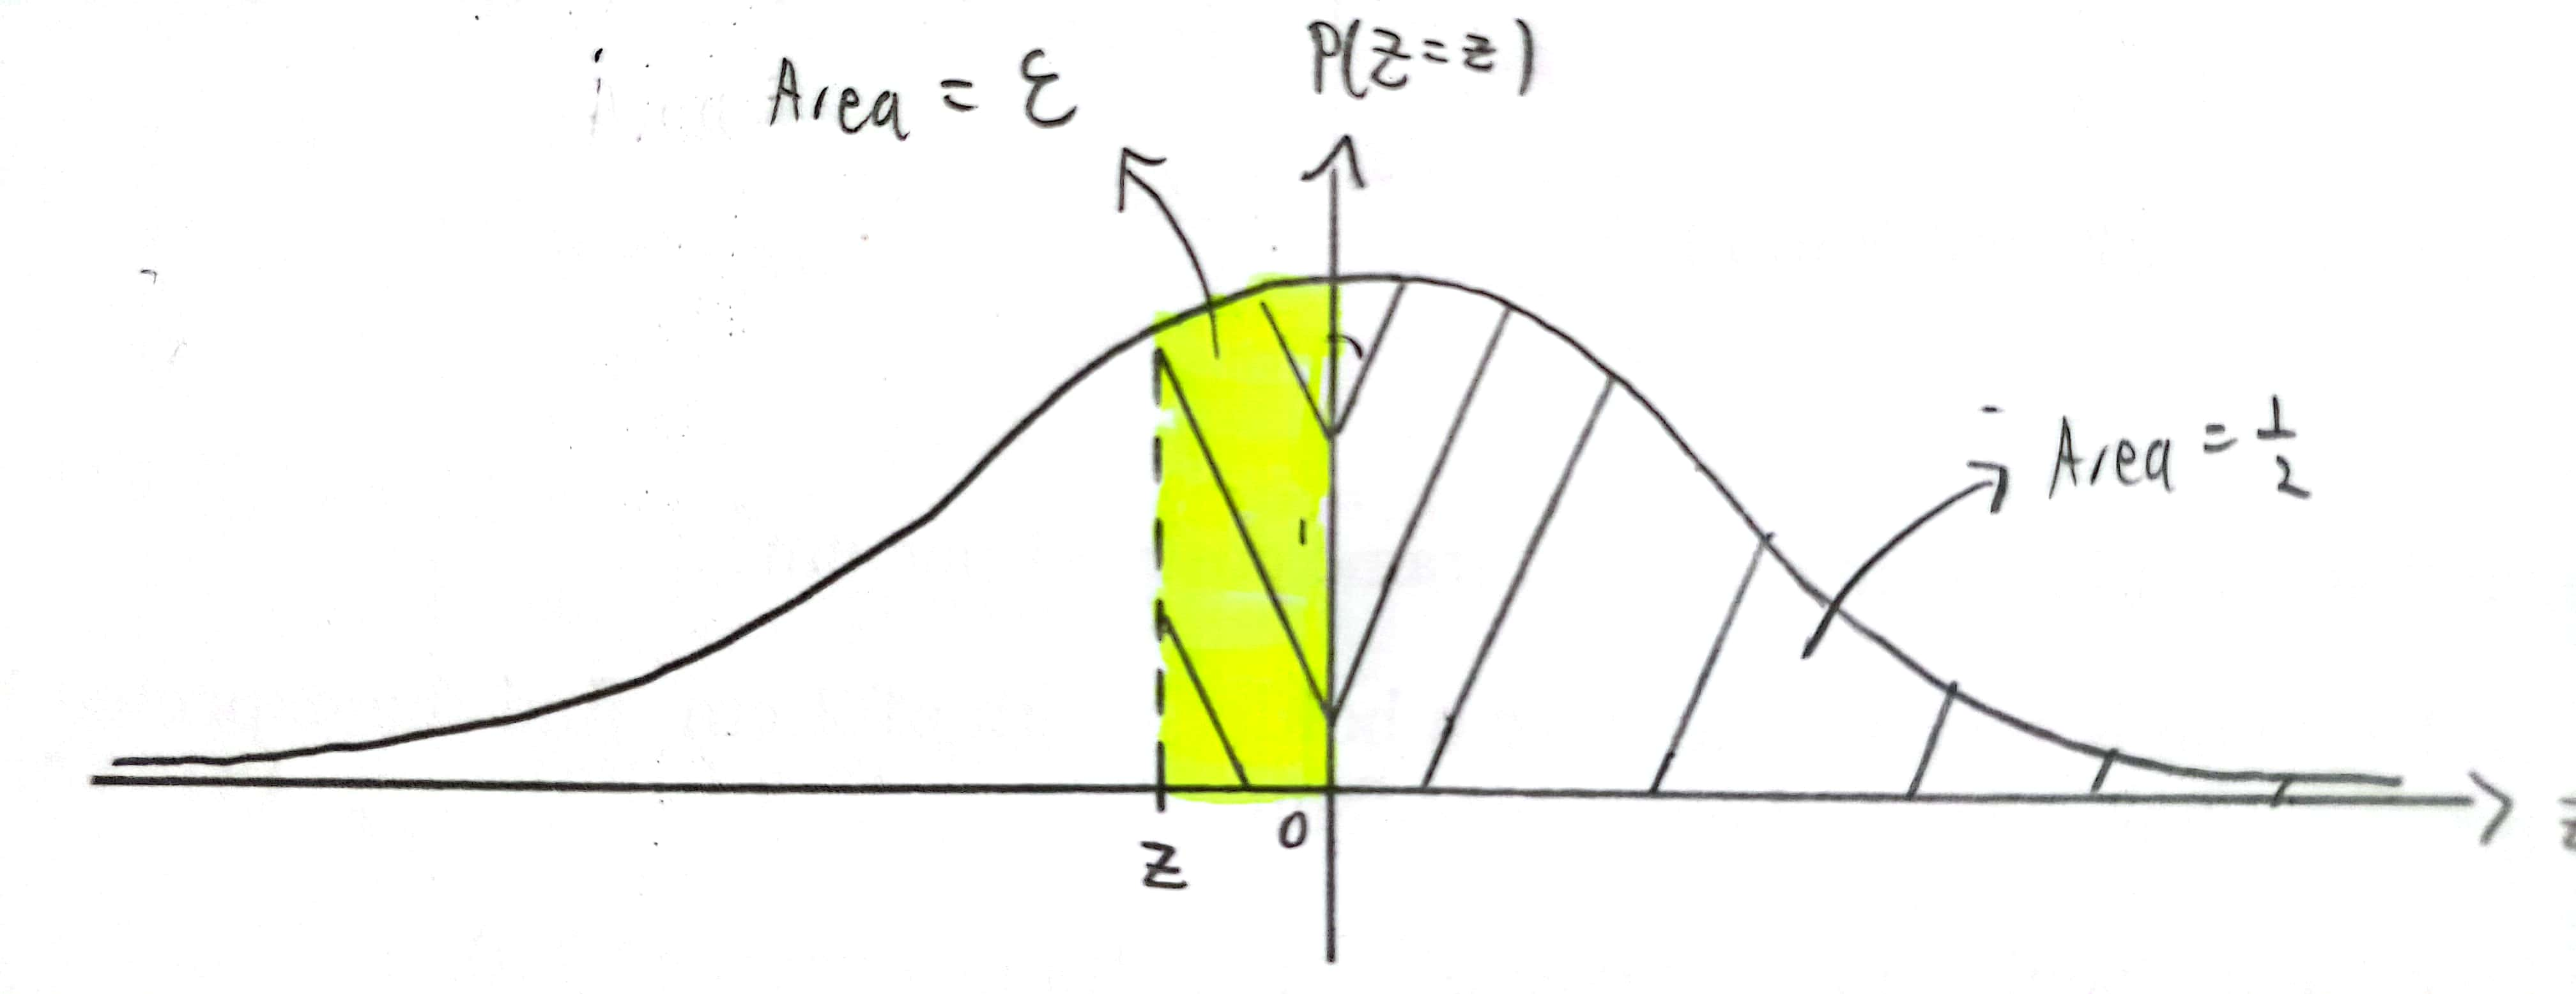
\includegraphics[width=\textwidth]{../images/Special-Continuous-Random-Variables-Example-Illustration.jpg}
  \end{center}
\end{example}
\begin{stbox}{}
  \begin{itemize}
    \setcounter{enumi}{7}
    \item A continuous random variable \(Y\) has an (negative) exponential distribution, which we denote with \(Y\sim \operatorname{Exp}(\lambda)\), iff its pdf \(g\) is such that
    \[g(Y)=
    \begin{cases}
      \lambda e^{-\lambda x} &\text{if \(x\geq 0\)}\\
      0 &\text{otherwise.}
    \end{cases}\]
    \item Expectation and variance:

    \begin{center}
      \begin{tabular}{|Sc|Sc|Sc|}
        \hline
        Distribution & Expectation & Variance\\
        \hline
        \(X\sim \operatorname{U}(a,b)\) & \(\dfrac{a+b}{2}\) & \(\dfrac{(b-a)^2}{12}\)\\
        \hline
        \(Y\sim \operatorname{Exp}(\lambda)\) & \(\dfrac{1}{\lambda}\) & \(\dfrac{1}{\lambda^2}\)\\
        \hline
      \end{tabular} 
    \end{center}
    \emph{Note}: We need to remember the expectation and variance for the uniform distribution, as it is not provided in the MF26 formula sheet (unlike all other distributions).
    \item \emph{Warning}: The G.C. tends to incorrectly process an integral if its upper and lower bounds contain \(\pm \text{E}99\).
  \end{itemize}
\end{stbox}
\chapter{Sampling and Estimation}
\begin{definition}{}{}
  A sample is a finite subset of the population.
\end{definition}
\begin{definition}{}{}
  A random sample is a sample selected such that each member of the population has an equal probability of being selected.
\end{definition}
\begin{definition}{}{}
  Any statistic \(T\) derived from a random sample and used to estimated an unknown population parameter \(\theta\) is known as an \emph{estimator}. It is an \emph{unbiased} estimator iff \(\E(T)=\theta\). If \(T\) is unbiased we commonly write \(\hat{\theta}\) for \(T\).
\end{definition}
\begin{stbox}{General Information}
  \begin{itemize}
    \item Either write \(\hat{\mu}\) or write out ``Unbiased estimate of the population mean \(\mu\), \(\widebar{x}=\dots\)'' Same holds for other population parameters \(\theta\).
    \item Estimators you should know:
    \item 
    % *A table where Parameter is under another column
    % \begin{center}
    %   \begin{tabular}{|Sc|Sc|Sc|Sc|Sc|}
    %     \hline
    %     \multicolumn{2}{|Sc|}{Parameter} & Estimator & Unbiased? & Formula\\
    %     \hline
    %     Population Mean & \(\mu\) & \(\widebar{X}\) & \checkmark & \(\dfrac{X_1+X_2+\dots+X_n}{n}\)\\
    %     \hline
    %     \multirow{2}{*}[-1.2cm]{Population Variance} & \multirow{2}{*}[-1.2cm]{\(\sigma^2\)} & \(\sigma_n^2\) & \(\times\) & 
    %     \begin{minipage}{3cm}
    %       \begin{center}
    %         \(\dfrac{\sum{(X_i-\widebar{X})^2}}{n}\)\\[1mm]
    %         \(\dfrac{\sum{X_i^2}}{n}-\widebar{X}^2\)
    %       \end{center}
    %     \end{minipage}\\
    %     \cline{3-4}
    %     & & \(S^2\) & \checkmark & 
    %     \begin{minipage}{5cm}
    %       \begin{center}
    %       \(\dfrac{n}{n-1}\sigma_n^2\)\\[1mm]
    %       \(\dfrac{\sum(X_i-\widebar{X})^2}{n-1}\)\\[1mm]
    %       \(\dfrac{1}{n-1}\left[ \sum X_i^2-\dfrac{(\sum X_i)^2}{n} \right]\)
    %       \end{center}
    %     \end{minipage}\\
    %     \hline
    %     Population Proportion & \(p\) & \(P_s\) & \checkmark & \(\dfrac{X}{n}\)\\
    %     \hline
    %   \end{tabular}
    % \end{center}
    \begin{center}
      \resizebox{0.94\textwidth}{!}{\begin{tabular}{|Sc|Sc|Sc|Sc|}
        \hline
        Parameter & Estimator & Unbiased? & Formula\\
        \hline
        Population Mean \(\mu\) & Sample Mean \(\widebar{X}\) & \checkmark & \(\dfrac{X_1+X_2+\dots+X_n}{n}\)\\
        \hline
        \multirow{2}{*}[-1.2cm]{Population Variance \(\sigma^2\)} & Sample Variance \(\sigma_n^2\) & \(\times\) & 
        \begin{minipage}{3cm}
          \begin{center}
            \(\dfrac{\sum{(X_i-\widebar{X})^2}}{n}\)\\[1mm]
            \(\dfrac{\sum{X_i^2}}{n}-\widebar{X}^2\)
          \end{center}
        \end{minipage}\\
        \cline{2-4}
        & \(S^2\) & \checkmark & 
        \begin{minipage}{5cm}
          \begin{center}
          \(\dfrac{n}{n-1}\sigma_n^2\)\\[1mm]
          \(\dfrac{\sum(X_i-\widebar{X})^2}{n-1}\)\\[1mm]
          \(\dfrac{1}{n-1}\left[ \sum X_i^2-\dfrac{(\sum X_i)^2}{n} \right]\)
          \end{center}
        \end{minipage}\\
        \hline
        Population Proportion \(p\) & Sample Proportion \(P_s\) & \checkmark & \(\dfrac{X}{n}\)\\
        \hline
      \end{tabular}}
    \end{center}
    \item Let \(X\) be a random variable following \emph{any distribution}, and suppose we have a random sample \(X_1,X_2,\dots,X_n\) of size \(n\geq 50\).
    
    Then by CLT (Central Limit Theorem), since \(n\geq 50\) is large, 
    \[\widebar{X}\sim \Normal\left(\mu,\frac{\sigma^2}{n}\right) \qquad\text{and}\qquad X_1+X_2+\dots+X_n\sim \Normal(n\mu,\nu\sigma^2)\]
    \emph{approximately}.
    \item Assumptions when using CLT:
    \begin{itemize}
      \item The sample is random.
      \item Each \(X_i\) is independent and identically distributed.
    \end{itemize}
    \item Suppose \(X\sim \Normal(\mu,\sigma^2)\) is known and we pick a \emph{particular} sample. Let the unbiased estimates for the population mean and variance of this sample be \(\widebar{x}\) and \(s^2\), respectively. Then,
    \begin{center}
      \begin{tabular}{|Sc|Sc|Sc|}
        \hline
        Distribution & Is An Approximation?\\
        \hline
        \(\widebar{X} \sim \Normal(\mu,\sigma^2)\) & No\\
        \hline
        \(\widebar{X} \sim \Normal(\widebar{x},\sigma^2)\) & Yes\\
        \hline
        \(\widebar{X} \sim \Normal(\mu,s^2)\) & Yes\\
        \hline
        \(\widebar{X} \sim \Normal(\widebar{x},s^2)\) & Yes\\
        \hline
      \end{tabular}
    \end{center}
    % ADD NAMES of the parameters and estimators to previous table
    So, if we obtain any of the latter three in solving a question, we must write ``\(X\sim \Normal(\rule{3mm}{0.1mm},\rule{3mm}{0.1mm})\)approximately'' (even though we knew \(X\) \emph{exactly} follows a normal distribution!)
    \item Pooled estimators you should know. First assume we have two populations, from which we select a random sample of size \(n_1\) and \(n_2\). We let \(\widebar{X}_1\) and \(S_1^2\) denote the sample mean and unbiased estimator for variance, respectively. Similarly define \(\widebar{X}_2\) and \(S_2^2\).
    \begin{center}
      \begin{tabular}{|Sc|Sc|}
        \hline
        Parameter & Unbiased Pooled Estimator\\
        \hline
         Mean  & \(\hat{\mu}=\dfrac{n_1\widebar{X}_1+n_2\widebar{X}_2}{n_1+n_2}\)\\
         \hline
         Variance & \(S_p^2=\dfrac{(n_1-1)S_1^2+(n_2-1)S_2^2}{n_1+n_2-2}\)\\
         \hline
      \end{tabular}
    \end{center}
    \item Let \(0<\alpha<1\)
  \end{itemize}
\end{stbox}
The following definition is found in 
\href{https://www.amazon.com/Introduction-Mathematical-Statistics-8th-Whats-dp-0134686993/dp/0134686993/ref=dp_ob_title_bk}{Hogg-McKean-Craig}. Similar definitions are also found in 
\href{https://www.amazon.sg/Mathematical-Statistics-Applications-William-Mendenhall/dp/0495110817#customerReviews}{Wackerly-Mendenhall-Schaefer}
and \href{https://www.amazon.com/Probability-Statistical-Inference-Statistics-Monographs/dp/0824703790}{Nitis Mukhopadhyay}.
\begin{definition}{}{}
  Let \(X_1,X_2,\dots,X_n\) be a sample on a random variable \(X\), where \(X\) has pdf \(f(x;\theta)\), \(\theta \in \Omega\). Let \(0<\alpha<1\) be specified. Let \(L=L(X_1,X_2,\dots,X_n)\) and \(U=U((X_1,X_2,\dots,X_n))\) be two statistics. We say that the interval \((L,U)\) is a \((1-\alpha)100\%\) \emph{confidence interval} for \(\theta\) iff 
  \[1-\alpha=P_\theta[\theta \in (L,U)].\]
  That is, the probability that the interval contains \(\theta\) is \(1-\alpha\), which is called the \emph{confidence coefficient} or \emph{confidence level} of the interval.
\end{definition}
\begin{stbox}{}
  \begin{itemize}
    \item We cannot write ``a \(1-\alpha\) (e.g. 0.95) confidence interval''. The \(1-\alpha\) must always be expressed as a \emph{percentage}.
    % \item Let \(0<\alpha<1\) and \(X_1,X_2,\dots,X_n\) be a sample on a random variable \(X\). Suppose \(n\) is large (\(n\geq 50\)). Then, CLT allows us to obtain the approximation
    % \[\frac{\widebar{X}-\mu}{\frac{S}{\sqrt{n}}}=Z\sim \Normal(0,1).\]
    % Rewriting \(\Prob(-z_{1-\alpha/2}<Z<z_{1-\alpha/2})=1-\alpha\) gives
    % \[\Prob\left( \widebar{x}-z_{1-\alpha/2}\frac{s}{\sqrt{n}}<\mu<\widebar{x}+z_{1-\alpha/2}\frac{s}{\sqrt{n}}\right)=1-\alpha.\] 
    % As such, a \((1-\alpha)100\%\) confidence interval is
    % \[\left( \widebar{x}-z_{1-\alpha/2}\frac{s}{\sqrt{n}}\,,\ \widebar{x}+z_{1-\alpha/2}\frac{s}{\sqrt{n}} \right).\]
    % When the variance \(\sigma^2\) is known, we can replace \(s\) with \(\sigma\).
    \item Let \(\hat{\theta}\) be a statistic that is normally distributed with mean \(\theta\) and standard error \(\sigma_{\hat{\theta}}\). We see that 
    \[\frac{\hat{\theta}-\theta}{\sigma_{\hat{\theta}}}=Z \sim \Normal(0,1).\]
    Rewriting \(\Prob(-z_{1-\alpha/2}<Z<z_{1-\alpha/2})=1-\alpha\) gives
    \[\Prob(\hat{\theta}-z_{1-\alpha/2}\sigma_{\hat{\theta}}<\theta<\hat{\theta}+z_{1-\alpha/2}\sigma_{\hat{\theta}})=1-\alpha.\]
    Hence, a \((1-\alpha)100\%\) confidence interval for \(\theta\) is
    \[(\hat{\theta}-z_{1-\alpha/2}\sigma_{\hat{\theta}}\,,\ \hat{\theta}+z_{1-\alpha/2}\sigma_{\hat{\theta}}).\]
    \href{https://www.amazon.sg/Mathematical-Statistics-Applications-William-Mendenhall/dp/0495110817#customerReviews}{(Wackerly-Mendenhall-Schaefer)}
    \item Let \(0<\alpha<1\) and \(X_1,X_2,\dots,X_n\) be a sample on a random variable \(X\) with mean \(\mu\), where \(n\) is large. Then, an approximate \((1-\alpha)100\%\) confidence interval for \(\mu\) is
    \[\left( \widebar{x}-z_{1-\alpha/2}\frac{s}{\sqrt{n}}\,,\ \widebar{x}+z_{1-\alpha/2}\frac{s}{\sqrt{n}} \right).\]
    When the variance \(\sigma^2\) is known, we can replace \(s\) with \(\sigma\). If the distribution of \(X\) is known to be normal, in addition to \(\sigma^2\) being known exactly, then the confidence interval is exact; it is not just an approximation. 

    \href{https://www.amazon.com/Introduction-Mathematical-Statistics-8th-Whats-dp-0134686993/dp/0134686993/ref=dp_ob_title_bk}{(Hogg-McKean-Craig)}
    \item Let \(X\) be a Bernoulli random variable with probability of success \(p\), where \(X\) is 1 or 0 if the outcome is success or failure, respectively. Suppose \(X_1,X_2,\dots,X_n\) is a random sample from the distribution of \(X\), where \(n\) is large. Let \(\hat{p}=\widebar{X}\) be the sample proportion of successes. Then, an approximate \((1-\alpha)100\%\) confidence interval for \(p\) is given by 
    \[\left( \hat{p}-z_{1-\alpha/2}\sqrt{\frac{\hat{p}(1-\hat{p})}{n}}\,,\ \hat{p}+z_{1-\alpha/2}\sqrt{\frac{\hat{p}(1-\hat{p})}{n}} \right).\]
    (Letting \(Y=X_1+X_2+\dots+X_n\sim \operatorname{B}(n,p)\) gives \(\hat{p}=Y/n\), which is the phrasing used by the school's notes.) 

    \href{https://www.amazon.com/Introduction-Mathematical-Statistics-8th-Whats-dp-0134686993/dp/0134686993/ref=dp_ob_title_bk}{(Hogg-McKean-Craig)}
  \end{itemize}
\end{stbox}
\begin{note}
  Standard phrasing for the interpretation of a \((1-\alpha)100\%\) confidence interval \((a,b)\). 
  \begin{center}
    The probability that the interval \((a,b)\) contains the [\(\mu\) in context] is \(1-\alpha\).
  \end{center}
\end{note}
\begin{note}
  Standard phrasing for what is a \((1-\alpha)100\%\) confidence interval for \(\theta\)?
  \begin{center}
    It is an interval which has probability \(1-\alpha\) of containing the true value of \(\theta\).  
  \end{center}
\end{note}
\begin{note}
  Standard phrasing for whether mean/proportion in context has likely increased/decreased, when given suitable confidence intervals.
  \begin{enumerate}
    \item There is no conclusive result.

    Since the old and new \((1-\alpha)\%\) confidence intervals overlap, we are unable to conclude whether the [mean/proportion in context] has decreased or not. Hence, it is inconclusive from these figures on whether the [context (e.g. an awareness campaign)] has been effective.
    \item It has likely increased/decreased.
    
    The old \((1-\alpha)\%\) confidence interval is to the left/right of the new \((1-\alpha)\%\) confidence interval, such that they do not overlap. So, can conclude that the [mean/proportion in context] likely increased/decreased. Hence, these figures suggests that the [context (e.g. an awareness campaign)] has been effective.
  \end{enumerate}
\end{note}
\begin{GCSkills}{}
  Calculating statistics (i.e. \(\widebar{x}\), \(s\), etc) by G.C. given data for a sample.
  \begin{enumerate}
    \item Keying in the data: \texttt{stat} \(\Longrightarrow\) \texttt{1:Edit} \(\Longrightarrow\) Key in the data into one of the lists \(\texttt{L}_i\). 
    \item Calculating the statistic: \texttt{stat} \(\Longrightarrow\) \texttt{CALC} \(\Longrightarrow\) \texttt{1-Var Stats} (\texttt{List:}\(\texttt{L}_i\)) \(\Longrightarrow\) \texttt{Calculate}.
    \item Getting the statistic for further calculations: \texttt{vars} \(\Longrightarrow\) \texttt{5:Statistics} \(\Longrightarrow\) Select the desired statistic.
  \end{enumerate}
\end{GCSkills}
\begin{GCSkills}{}
  Calculating the symmetric confidence interval by G.C.
  \begin{center}
  \begin{tabular}{ll}
    Mean: & \texttt{stat} \(\Longrightarrow\) \texttt{TESTS} \(\Longrightarrow\) \texttt{7:ZInterval\dots}\\
    Proportion: & \texttt{stat} \(\Longrightarrow\)\texttt{TESTS} \(\Longrightarrow\) \texttt{A:1-PropZInt\dots}\\ 
  \end{tabular}
  \end{center}
\end{GCSkills}
\chapter{Correlation and Linear Regression}
\begin{note}
  A good scatter diagram should follow the guidelines below.
  \begin{itemize}
    \item The relative position of each point on the scatter diagram should be clearly shown.
    \item The range of values for the set of data should be clearly shown by marking out the extreme \(x\) and \(y\) values on the corresponding axis.
    \item The axes should be labeled clearly with the variables.
  \end{itemize}
\end{note}
\begin{stbox}{General Information}
  \begin{itemize}
    \item The Product Moment Correlation Coefficient is a measure of the linear correlation between two variables. It is defined by
    \[r=\frac{\sum{(x-\bar{x})(y-\bar{y})}}{\sqrt{\sum{(x-\bar{x})^2}\sum{(y-\bar{y})^2}}}=\frac{\sum{xy}-\dfrac{\sum{x}\sum{y}}{n}}{\sqrt{\left[\sum{x^2}-\dfrac{\left(\sum{x}\right)^2}{n}\right]\left[\sum{y^2}-\dfrac{\left(\sum{y}\right)^2}{n}\right]}},\]
    which takes on a value from 0 to 1.
    \item When \(r=0\), there is no linear relationship. But, a nonlinear relationship may be present. Additionally, the regression lines are perpendicular.
    \item The closer the value of \(r\) is to 1 (or -1), the stronger the positive (or negative) linear correlation. Furthermore, the regression lines coincide.
    \begin{center}
      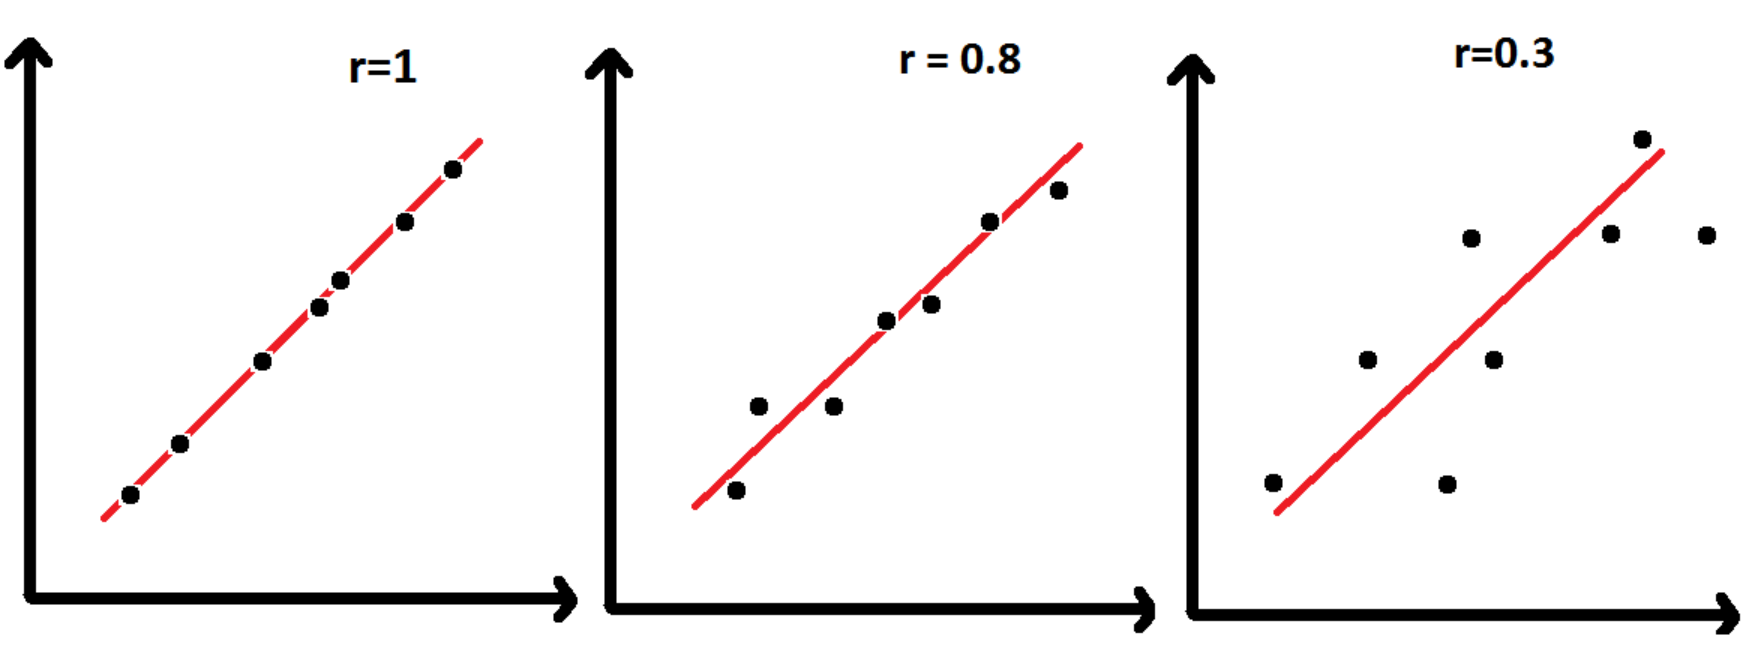
\includegraphics[scale=0.3]{../images/Product Moment Correlation Coefficient 1.png}
      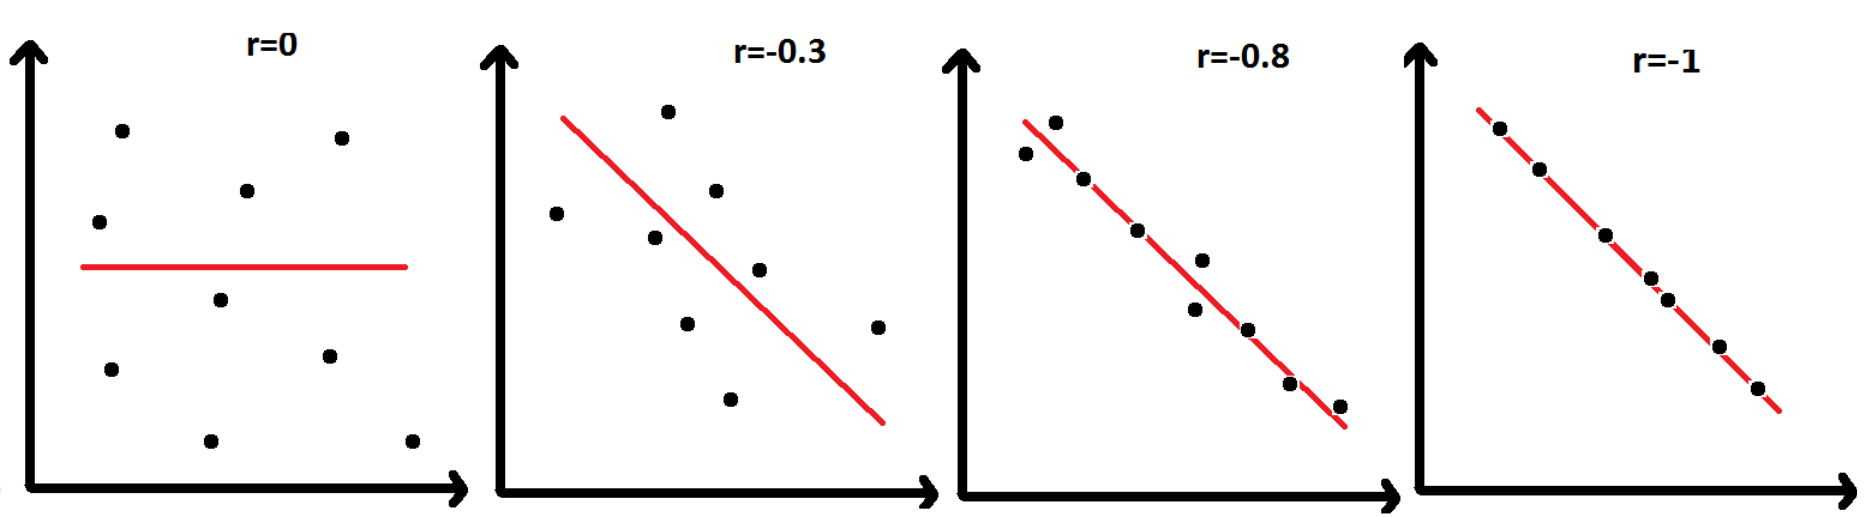
\includegraphics[scale=0.4]{../images/Product Moment Correlation Coefficient 2.png}
    \end{center}
    \item The regression line of \(y\) on \(x\) minimises the sum of squares deviation (error) in the \(y\)-direction. (i.e. we are assuming \(x\) is the independent variable whose values are known exactly.) It is given by
    \[y=\bar{y}+b(x-\bar{x}),\qquad\text{where}\qquad b=\frac{\sum{(x-\bar{x})(y-\bar{y})}}{\sum{(x-\bar{x})^2}}=\frac{\sum{xy}-\dfrac{\sum{x}\sum{y}}{n}}{\sum{x^2}-\dfrac{\left(\sum{x}\right)^2}{n}}.\] 
    \item The point \((\bar{x},\bar{y})\) always lies on both the regression lines of \(y\) on \(x\), and \(x\) on \(y\).
    \item Say we are given the value of one variable, and asked to approximate the the value of the other variable. Then, we should always use the line of the \emph{dependent} variable on the \emph{independent}.
    \item Estimations should not be taken for data outside the range of the sample provided, even if the value of \(r\) is close to 1.
  \end{itemize}
\end{stbox}
\end{document}